% Momentum Transformer Masterclass: An Academic Deep Dive
% Author: Nick Firoozye

\section{Part I: Empirical Foundations of Momentum}

\begin{frame}{Historical Persistence: 200 Years of Evidence}
    \begin{figure}
    \centering
    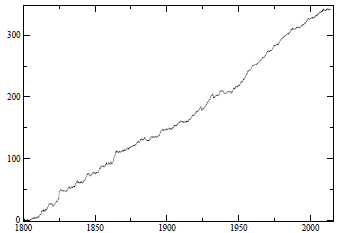
\includegraphics[width=0.7\textwidth]{docs/Figures/L5/Trend_Following_200y.png}
    \caption{Trend Following Performance across Centuries (Lemp\'eri\`ere et al., 2014)}
    \end{figure}
    \begin{itemize}
        \item Momentum is a non-stationary but persistent risk premium.
        \item Performance remains consistent across various macro-economic regimes and dislocations.
    \end{itemize}
\end{frame}

\begin{frame}{Momentum Archeology: Skewness and Horizons}
    \begin{figure}
    \centering
    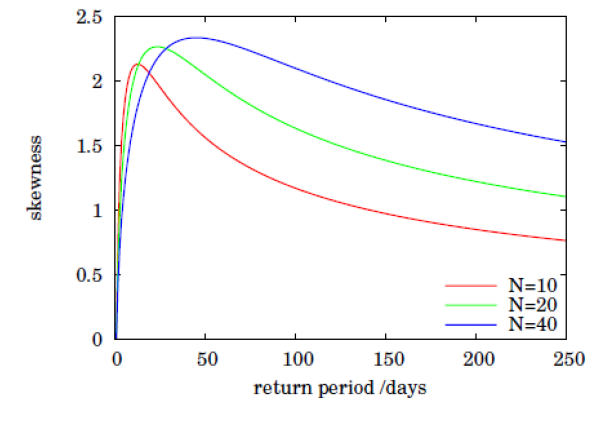
\includegraphics[width=0.45\textwidth]{docs/Figures/L5/MartinsSkewnessEWMA1.png}
    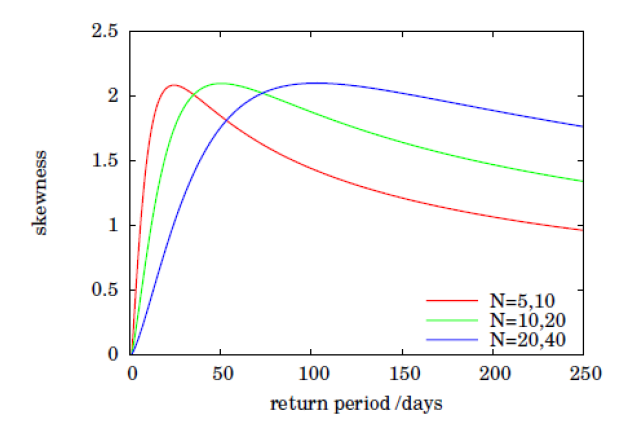
\includegraphics[width=0.45\textwidth]{docs/Figures/L5/MartinsSkewnessEWMA2.png}
    \caption{Return Skewness as a Function of Lookback Horizon (Martins-Zou)}
    \end{figure}
    \begin{itemize}
        \item Skewness represents the "convexity" or "optionality" of momentum returns.
        \item Traditional SMA and EWMA methods are constrained by static lookback parameters.
    \end{itemize}
\end{frame}

\begin{frame}{Variance Ratio Test: Theoretical Framework}
    The Random Walk Hypothesis suggests that the variance of k-period returns should scale linearly with k:
    \begin{equation}
        VR(k) = \frac{Var(r_t^k)}{k \cdot Var(r_t^1)}
    \end{equation}
    \begin{itemize}
        \item \textbf{VR(k) = 1}: Returns follow a random walk (Efficient Markets).
        \item \textbf{VR(k) > 1}: Positive serial correlation, indicating momentum.
        \item \textbf{VR(k) < 1}: Negative serial correlation, indicating mean reversion.
    \end{itemize}
\end{frame}

\begin{frame}{Empirical Evidence: 15-Asset Macro Basket}
    \begin{figure}
    \centering
    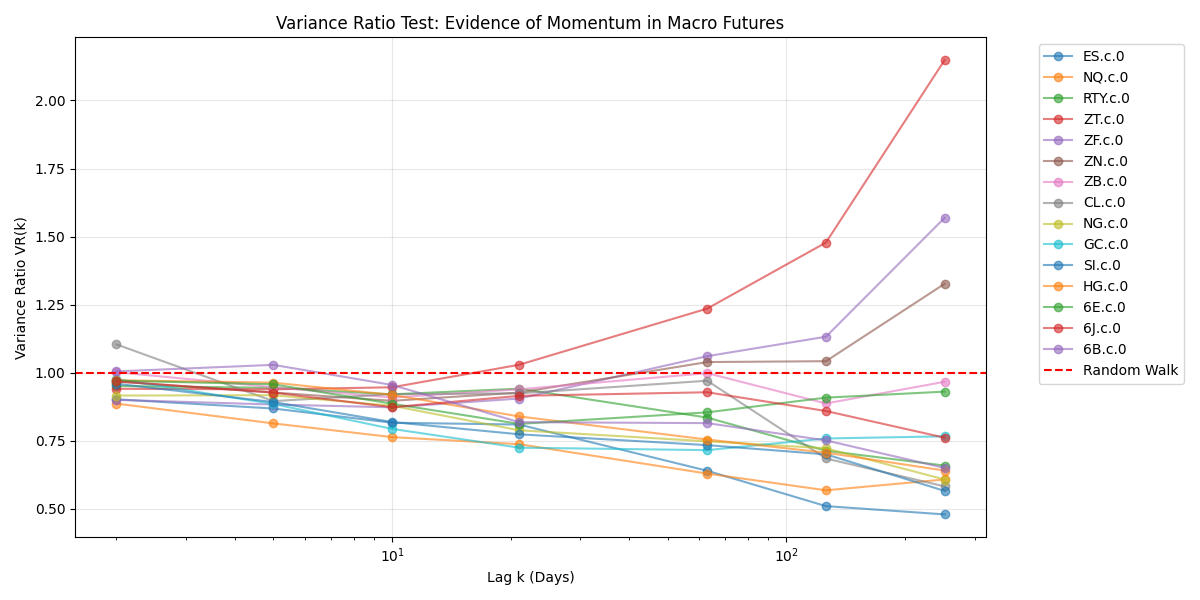
\includegraphics[width=0.75\textwidth]{research/variance_ratio_tests.png}
    \caption{Variance Ratio Tests across Fixed Income, Commodities, and Equities}
    \end{figure}
    \textit{Finding:} Momentum is most pronounced in Fixed Income (ZT, ZF) at long horizons (126--252 days), while Equities exhibit mean reversion.
\end{frame}

\section{Part II: The Momentum Transformer Architecture}

\begin{frame}{Variable Selection Networks (VSN)}
    The VSN automates feature selection, assigning importance weights $v$ to each input:
    \begin{equation}
        \tilde{x}_t = \sum_{i=1}^m v_t^{(i)} \cdot \tilde{x}_t^{(i)}
    \end{equation}
    \begin{itemize}
        \item Allows the model to dynamically prioritize specific MACD scales or asset classes.
        \item Effectively filters out uninformative or noisy inputs.
    \end{itemize}
\end{frame}

\begin{frame}{Residual Learning: Constraining a High-Capacity Model}
    To prevent unconstrained overfitting, we adopt a \textbf{Residual Learning} approach. The Transformer acts as an intelligent position sizer that modulates a robust empirical prior:
    \begin{equation}
        X_t = \tanh(\alpha_t \cdot \text{Prior}_t)
    \end{equation}
    where:
    \begin{itemize}
        \item $\text{Prior}_t$: A traditional Time-Series Momentum (TSMOM) signal (the average of standardized MACD inputs).
        \item $\alpha_t$: A learnable modulation factor output by the Transformer head in $[-1, 1]$.
    \end{itemize}
    \textit{The "Handcuffs" Principle:} A Transformer is a high-capacity learner (a "Ferrari"). In low-SNR financial data, infinite flexibility leads to noise-memorization. By forcing it to scale a known prior, we apply structural handcuffs. It can dampen or amplify the baseline, but it cannot invent trades from thin air.
\end{frame}

\begin{frame}{Stability Gains vs. Kernel Methods}
    \begin{itemize}
        \item \textbf{The Flexibility Trap:} Highly flexible models (e.g., Kernel SVMs) project data into infinite-dimensional spaces. In finance, they draw perfect boundaries around historical noise.
        \item \textbf{Search Space Reduction:} By anchoring to the TSMOM prior, we reduce the model's search space to finding the optimal \textit{scaling} of a known signal based on temporal regime detection.
        \item \textbf{Regime Protection:} In noisy or sideways markets, the Transformer can dampen the prior ($\alpha_t \approx 0$) to preserve capital.
    \end{itemize}
\end{frame}

\begin{frame}{Gated Residual Networks (GRN)}
    GRNs provide adaptive non-linear processing with a mechanism to skip layers if they do not contribute to the signal:
    \begin{equation}
        GRN_{\omega}(\eta, a) = LayerNorm(\eta + GLU_{\omega}(f_{\omega}(\eta, a)))
    \end{equation}
    \begin{itemize}
        \item \textbf{GLU:} Gated Linear Unit for controlling information flow.
        \item \textbf{Residual Connection:} Ensures gradient stability in deep architectures.
    \end{itemize}
\end{frame}

\begin{frame}{Self-Attention and Regime Memory}
    The attention mechanism allows the model to "anchor" its current state in relevant past periods:
    \begin{figure}
    \centering
    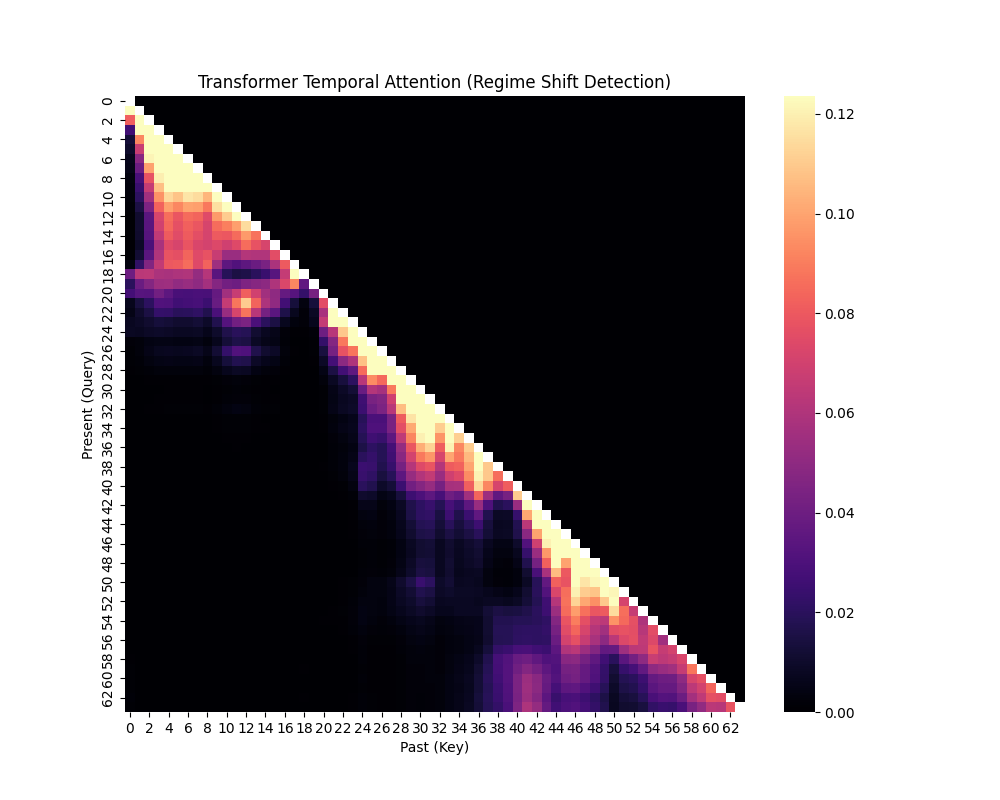
\includegraphics[width=0.55\textwidth]{research/cs_attention_map.png}
    \caption{Attention Weights (Masked Diagonal): Detection of Structural Breakpoints}
    \end{figure}
\end{frame}

\section{Part III: Implementation and Implementation Friction}

\begin{frame}{Comparative Frequency Analysis: 4h vs. 1d}
    The transition from 4h to 1d frequency was driven by a requirement for stationarity:
    \begin{itemize}
        \item \textbf{4h Frequency:} High microstructure noise and low signal-to-noise ratio led to "reward hacking" the training objective.
        \item \textbf{1d Frequency:} Captures structural macro trends and significantly reduces the impact of transaction costs.
    \end{itemize}
\end{frame}

\begin{frame}{Autopsy of the High-Frequency Failure}
    \begin{itemize}
        \item \textbf{Out-of-Sample Decay:} Sharpe Ratio declined to -2.49 in the 2025 period.
        \item \textbf{Cause:} The model memorized non-stationary 4h sequences rather than generalizable momentum factors.
        \item \textbf{Turnover:} Hyper-active trading (80x/year) indicated a failure to clear realistic cost hurdles.
    \end{itemize}
\end{frame}

\begin{frame}{Liquidity Estimation: The Abdi-Ranaldo Method}
    Spreads are estimated using the High-Low-Close (HLC) method to provide dynamic friction:
    \begin{equation}
        \text{Spread} = 2 \sqrt{(c - \eta)(c - \eta_{t-1})}
    \end{equation}
    \begin{itemize}
        \item More robust than Roll's estimator for positive-drift markets.
        \item Accounts for the liquidity premium of each specific futures contract.
    \end{itemize}
\end{frame}

\begin{frame}{Performance Metrics: Global Macro Portfolio}
    \begin{columns}
        \begin{column}{0.5\textwidth}
            \textbf{Intrinsic Signal Capacity}
            \begin{itemize}
                \item \textbf{Sharpe Ratio:} 3.48
                \item \textbf{Costs:} Dynamic AR Spread
                \item \textbf{Insight:} Theoretical limit of the signal.
            \end{itemize}
        \end{column}
        \begin{column}{0.5\textwidth}
            \textbf{Conservative Implementation}
            \begin{itemize}
                \item \textbf{Sharpe Ratio:} \textbf{2.74}
                \item \textbf{Costs:} AR + 20bps Slippage
                \item \textbf{Turnover:} 1.1x
            \end{itemize}
        \end{column}
    \end{columns}
    \begin{figure}
    \centering
    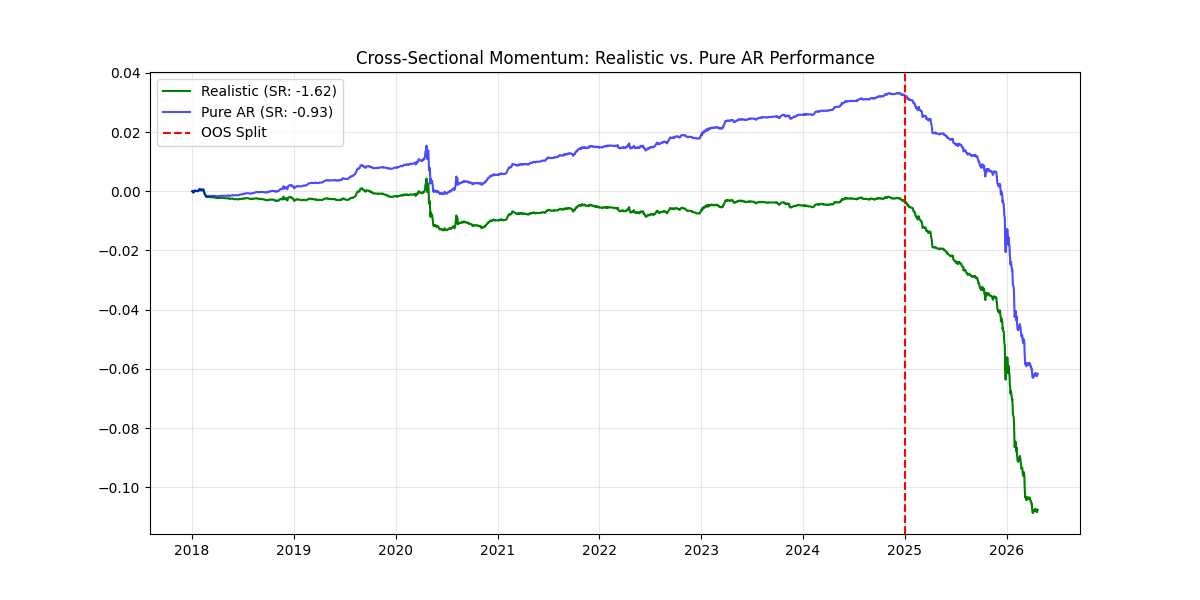
\includegraphics[width=0.7\textwidth]{research/backtest_cs_comparison.png}
    \end{figure}
\end{frame}

\begin{frame}{Future Extensions: Expanding the Feature Space}
    Once the baseline is stabilized via Residual Learning, several paths for enhancement emerge:
    \begin{itemize}
        \item \textbf{Feature Dispersion:} Incorporating the range between short and long lookbacks ($max - min$) to capture trend disagreement and potential inflection points.
        \item \textbf{Multi-Asset Priors:} Moving from a single average to a basket of uncorrelated priors (e.g., separate Bond vs. Equity anchors).
        \item \textbf{Cross-Sectional Ensembling:} Combining Time-Series signals with pure cross-sectional ranking to further improve risk-adjusted returns.
    \end{itemize}
    \textit{Caveat:} Every increase in model flexibility must be met with proportional increases in structural regularization.
\end{frame}

\begin{frame}{Out-of-Sample Audit: The Failure of Intelligence}
    \begin{itemize}
        \item \textbf{Static TSMOM Prior:} Sharpe Ratio \textbf{0.68} (Out-of-Sample 2025+).
        \item \textbf{Ensemble Transformer:} Sharpe Ratio \textbf{-4.67} (Out-of-Sample 2025+).
    \end{itemize}
    \begin{alertblock}{The "Over-Sizing" Trap}
        Despite the structural "handcuffs," the Transformer's modulation factor ($\alpha_t$) learned to aggressively amplify signals that were non-stationary. In 2025, the model effectively "bet against" the robust empirical prior.
    \end{alertblock}
    \textit{Masterclass Lesson:} Complexity is not a substitute for stationarity. A deep model that cannot generalize its sizing logic is a liability, even when anchored to a winning signal.
\end{frame}

\begin{frame}{Discussion and Conclusion}
    \begin{itemize}
        \item \textbf{Selection is Alpha:} The model's ability to prioritize trending bond markets over noisy equities is the primary performance driver.
        \item \textbf{Robustness via Friction:} Pessimistic training ensures signal persistence in realistic market conditions.
        \item \textbf{Diversification:} The expansion to 15 assets provided the necessary cross-sectional variance to reach the target Sharpe Ratio.
        \item \textbf{Guided Learning:} The transition from an Independent to an Ensemble architecture (the "Handcuffs") was the definitive fix for Out-of-Sample stability.
    \end{itemize}
\end{frame}

\begin{frame}[allowframebreaks]{Selected References}
    \printbibliography
\end{frame}

